\documentclass[a4paper,10pt]{article}
\usepackage{amsmath,amssymb,graphicx,float,subfig}

%defines
\def\bY{{\bf Y}}
\def\bA{{\bf A}}
\def\bB{{\bf B}}
\def\bX{{\bf X}}
\def\bH{{\bf H}}
\def\bE{{\bf E}}
\def\bG{{\bf G}}
\def\bV{{\bf V}}
\def\bQ{{\bf Q}}
\def\btQ{{\bf \tilde Q}}
\def\bC{{\bf C}}
\def\btA{{\bf \tilde A}}
\def\b1{{\bf 1}}
\def\bx{{\bf x}}
\def\bb{{\bf b}}
\def\be{{\bf e}}
\def\by{{\bf y}}
\def\bz{{\bf z}}
\def\btx{{\bf{\tilde x}}}
\def\blambda{{\boldsymbol \lambda}}
\def\bgamma{{\boldsymbol \gamma}}
\def\btheta{{\boldsymbol \theta}}
\def\bbeta{{\boldsymbol \beta}}
\def\bnu{{\boldsymbol \nu}}
\def\bmu{{\boldsymbol \mu}}
\def\sigmaeps{{\sigma_{\epsilon}}}

%opening
\title{Home Assignment - 2}
\author{Santhosh Nadig}

\begin{document}

\maketitle

\section{Introduction}


\section{The Data-Set and Model}
The data consists of precipitation for the month of June, 2011 for 553 locations in the Parana district of Brazil. In addition, we are given the co-ordinates (latitude, longitude), elevation and distance to the coast are provided. The data is positive (since it is the accumulated precipitation) and the following model is suggested.

\begin{itemize}
 \item The observations $y_i$ are Gamma distributed
 \begin{align*}
  & y_i|z_i \sim \Gamma \left( b , \frac{e^{z_i}}{b}\right) \\
  & p(y_i|z_i) = \frac{y_i^{b-1}}{\Gamma(b)} \left( b e^{-z_i} \right)^b \exp(b y_i e^{-z_i})
 \end{align*}
 The mean $E(y_i|z_i) = e^{z_i}$ and $\log E(y_i|z_i) = z_i$. And, the variance $V(y_i|z_i) = e^{2z_i}/b$.
 
 \item The log-expectation of the observations $\bz$ is modeled as 
 \begin{align*}
  & \bz = \bA \bx + \bB \bbeta = \btA \btx.
 \end{align*}
 where $\bA$ is the observation matrix, $\bB$ is a matrix of covariates and
 \begin{align*}
  &\btx = \begin{bmatrix}
          \bx \\
          \bbeta
         \end{bmatrix} \sim
         N\left( 0, \begin{bmatrix}
                     \bQ & 0 \\
                     0 & \mathbb{I} \cdot 10^{-3}
                    \end{bmatrix}^{-1}
 \right)
 \end{align*}
 \item A suitable model for $\bQ$ is a SAR model: $\bQ = \tau (\kappa^4 \bC + 2\kappa^2 \bG + \bG_2)$ with parameters $\theta_1 = \log (\tau)$,  $\theta_2 = \log (\kappa^2)$  and $\theta_3 = \log(b)$.
\end{itemize}


\section{Theory}
\subsection{Observation Log-Likelihood}
The data model is given by
\begin{equation*}
 p(y_i|z_i) = \frac{y_i^{b-1}}{\Gamma(b)} (be^{-z_i})^b \exp (-by_ie^{-z_i}).
\end{equation*}
Thus, the observation log-likelihood $\log p(y_i|z_i)$ can be written as
\begin{equation*}
 f(z_i) \triangleq \log p(y_i|z_i) = (b-1) \log y_i - \log \Gamma(b) + b \log (b) - b z_i - b y_i e^{-z_i},
\end{equation*}
whose derivatives are
\begin{align*}
 f'(z_i) &= -b + b z_i y_i e^{-z_i} \\
 f''(z_i) &= b y_i e^{-z_i} (1 - z_i) .
\end{align*}

\subsection{Log-likelihood $\log p(\btx|\by, \btheta)$}
The log-likelihood function $\log p(\btx|\by, \btheta)$ can be written as
\begin{align}
 \log p(\btx|\by, \btheta) &\propto \log p(\by| \btx, \btheta) + \log p(\btx|\btheta) + \mathrm{const.} \nonumber \\
 &= \sum_i \log p(y_i|z_i, \btheta) + \log p(\btx|\btheta) + \mathrm{const.} \nonumber \\
 &= \sum_i f(z_i) - \frac{1}{2} \btx^T \bQ \btx  + \mathrm{const.}
 \label{eq:logpxyt}
\end{align}
The Taylor expansion around the mode $\hat \bx^{(0)}$ of the first term $\sum_i f(z_i)$ is given by [slide 29 of lecture 7]
\begin{equation}
 \sum_i f(z_i) \approx \mathrm{const.} + \btx^T \btA^T (\nabla f^{(0)} - \bH_f^{(0)} \btA \hat \bx^{(0)}) + \frac{1}{2} \btx^T \btA^T \bH_f^{(0)} \btA \btx
 \label{eq:taylor}
\end{equation}
where $\nabla f^{(0)}$ and $\bH_f^{(0)}$ represent the gradient and Hessian of $f$ at the mode of $\btx$.
Substituting (\ref{eq:taylor}) in (\ref{eq:logpxyt}), one obtains
\begin{equation}
 g(\btx) \triangleq \log p(\btx|\by, \btheta) \approx \btx^T \bb_{x|y} - \frac{1}{2} \btx^T \bQ_{x|y} \btx,
 \label{eq:gx}
\end{equation}
where $\bb_{x|y} = \btA^T (\nabla f^{(0)} - \bH_f^{(0)} \btA \hat \bx^{(0)})$ and $\bQ_{x|y} = \btQ - \btA^T \bH_f^{(0)} \btA$.

Taking the first derivative w.r.t $\btx$ of (\ref{eq:gx}), one obtains
\begin{align}
 g'(\btx) &= \btA^T (\nabla f^{(0)} - \bH_f^{(0)} \btA \hat \bx^{(0)}) - (\btQ - \btA^T \bH_f^{(0)} \btA) \btx \nonumber \\
	  &= \btA^T \nabla f^{(0)} - \btQ \hat \bx^{(0)} \qquad \mathrm{at~} \btx = \hat \bx^{(0)}.
\end{align}
The second derivative w.r.t $\btx$ of (\ref{eq:gx}) can simply be written as
\begin{equation}
 g''(\btx) = -(\btQ - \btA^T \bH_f^{(0)} \btA).
\end{equation}

\section{Estimation}
The observations are divided into estimation and validation data-sets wherein approximately 10\% of the observations are set aside for validation.
\subsection{Ordinary Least Squares}
The model for ordinary least squares is given by
\begin{equation*}
 \bz = \bB \bbeta + \be
\end{equation*}
where $\bB$ represents the matrix of covariates, $\bbeta$ the vector of coefficients and $\be \sim N(0,\sigmaeps^2)$.

The first step is to select a suitable set of covariates. Towards this end, a set of models tabulated in table \ref{tab:models} are explored.
\begin{table}[H]
\centering
\begin{tabular}{lp{9cm}}
\hline
{\bf Model} & {\bf Covariates} \\
\hline
 A & Latitude, longitude, distance to coast, elevation\\
 * B & Latitude, distance to coast, elevation\\
 C & Distance to coast, elevation\\
 D & Longitude, distance to coast\\
 E & Longitude, elevation\\
\hline
\end{tabular}
\caption{Models and the respective covariates, with log precipitation as the independent varible.}
\label{tab:models}
\end{table}

The standard error of the residuals and Akaike Information Criterion (AIC) for the models are shown in figure \ref{fig:aicse}. Clearly, model B is the best choice. Thus, the covariates include an intercept ($\beta_0$), latitude, distance to coast and elevation.
\begin{figure}[ht]
\centering
  \subfloat[]{{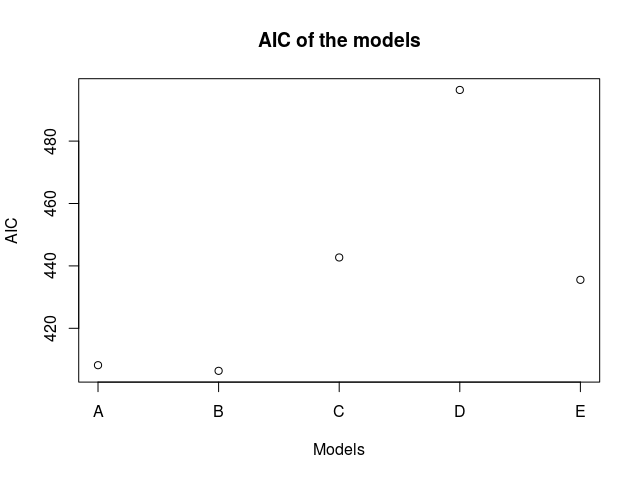
\includegraphics[width=5cm, height=5cm]{AIC_mm.png} }}%
  \qquad
  \subfloat[]{{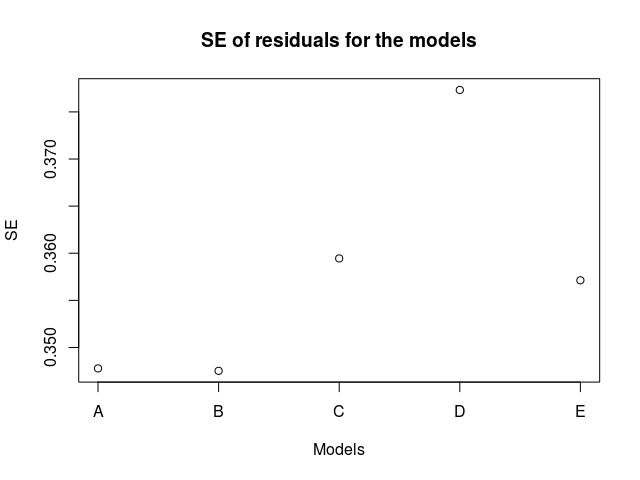
\includegraphics[width=5cm, height=5cm]{SE_Resid_mm.png} }}%
  \caption{(a): AIC (b): SE of residuals.}
\label{fig:aicse}
\end{figure}

The estimated parameters $\hat \bbeta$ and their corresponding standard errors tabulated in table~\ref{tab:olsparest}. The estimated noise variance was $\sigmaeps^2 = 0.1069$.
\begin{table}[H]
\centering
\begin{tabular}{lll}
\hline
{\bf Parameter} & {\bf Estimate} & {\bf SE} \\
\hline
$\hat \beta_0$ & -10.8703 & 1.9788 \\
$\hat \beta_1$ & -0.2430 & 0.0413 \\
$\hat \beta_2$ & -0.2234 & 0.0429 \\
$\hat \beta_3$ & 0.0006 & 0.0001 \\
\hline
\end{tabular}
\caption{OLS parameter estimate and standard errors.}
\label{tab:olsparest}
\end{table}

The OLS estimate of the precipitation at the validation locations is simply given by $\hat \by_v = \exp \left( \bB_v \hat \bbeta \right)$, where $\bB_v$ is the covariate matrix for the validation locations. Furthermore, the variance of the estimates is given by $\bV(\hat \by_v) = \sigmaeps^2 (\bB_v (\bB_v^T\bB_v)^{-1} \bB_v^T + 1)$. The 95\% confidence intervals (Gaussian) are given by $\hat \by_v \pm 1.96 \left( \bV(\hat \by_v) \right)^{1/2}$.

The OLS estimate for the validation locations, along with the 95\% confidence intervals are plotted in figure~\ref{fig:valid} (a).
\begin{figure}[ht]
\centering
  \subfloat[]{{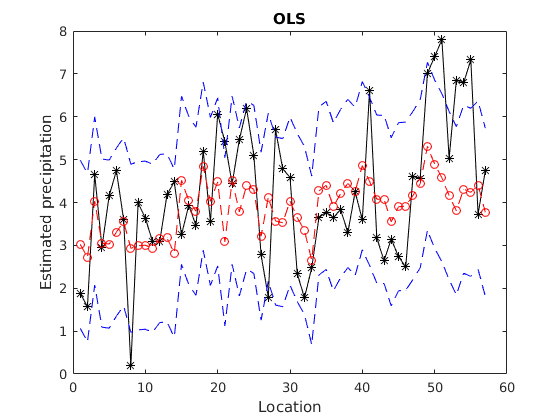
\includegraphics[width=5cm, height=5cm]{ols_valid.png} }}%
  \qquad
  \subfloat[]{{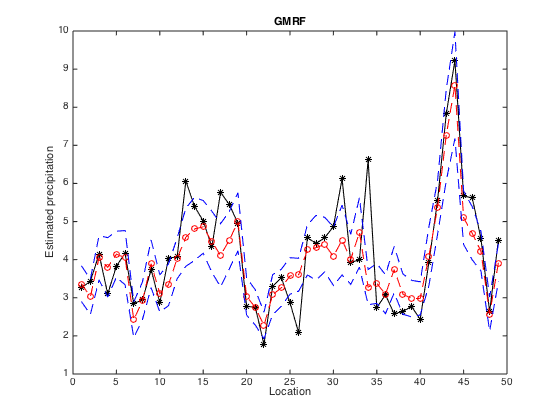
\includegraphics[width=5cm, height=5cm]{gmrf_valid.png} }}%
  \caption{(a): OLS estimate of precipitation at the validation locations. Black: Truth, Red: OLS estimate, Blue: 95\% confidence intervals. (b): GMRF estimate of precipitation at the validation locations. Black: Truth, Red: OLS estimate, Blue: 95\% confidence intervals.}
\label{fig:valid}
\end{figure}

\begin{verbatim}

sigma2 = 0.1069

theta =

    0.5522
    0.0205
    2.5509

exp(theta)

ans =

    1.7370
    1.0207
   12.8187
   
>> th_se

th_se =

    1.0012
    1.0004
    1.0003
\end{verbatim}

\subsection{Gaussian Markov Random Field (GMRF)}
Model is as described in section .

We begin by estimating the parameters. The parameter estimates are obtained by maximizing the posterior $p(\btheta|\by)$. That is,
\begin{equation*}
 \hat \btheta = \arg\max_{\btheta} \, p(\btheta|\by)
\end{equation*}
Since we assume $p(\btheta) \propto 1$ (``flat-prior''), we may express the posterior as
\begin{align*}
 p(\btheta|\by) \propto p(\by|\btheta) &= \frac{p(\by|\btx, \btheta) p(\btx|\btheta)}{p(\btx|\by, \btheta)} \\
 &= \frac{p(\by|\btx, \btheta) p(\btx|\btheta)}{p_G(\btx|\by, \btheta)}
\end{align*}

\begin{figure}[ht]
\centering
  \subfloat[]{{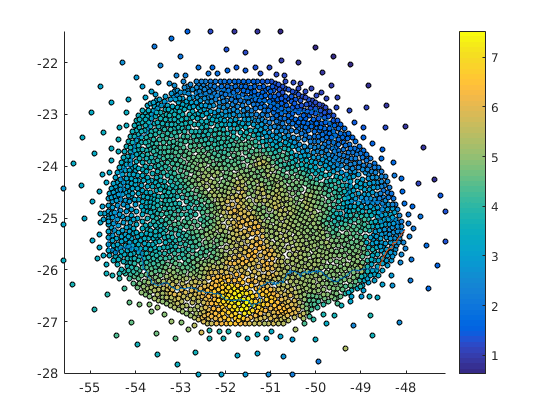
\includegraphics[width=5cm, height=4cm]{mesh_pred.png} }}%
  \qquad
  \subfloat[]{{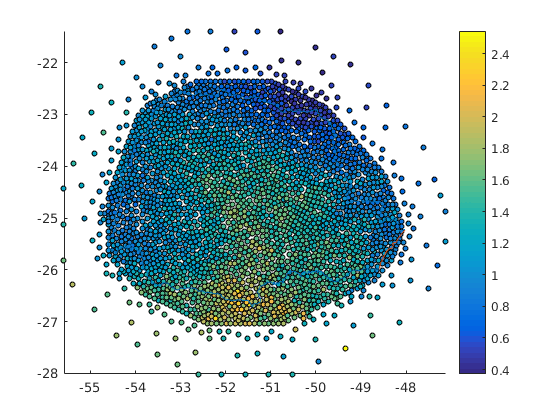
\includegraphics[width=5cm, height=4cm]{mesh_se.png} }}%
  \caption{(a): Prediction (mesh), (b): SE of predictions.}
\label{fig:mesh}
\end{figure}
\section{Conclusions}

\end{document}
